%----------------------------------------------------------------------------------------
%	PACKAGES AND OTHER DOCUMENT CONFIGURATIONS
%----------------------------------------------------------------------------------------

\documentclass[paper=a4, fontsize=11pt]{scrartcl} % A4 paper and 11pt font size

\usepackage[T1]{fontenc} % Use 8-bit encoding that has 256 glyphs
\usepackage{fourier} % Use the Adobe Utopia font for the document - comment this line to return to the LaTeX default
\usepackage[english]{babel} % English language/hyphenation
\usepackage{amsmath,amsfonts,amsthm, amssymb} % Math packages
\usepackage[utf8]{inputenc}
\usepackage[backend=bibtex, sorting=none]{biblatex}
\addbibresource{references.bib}
\usepackage{hyperref}
\usepackage{url}

\usepackage{graphicx}
\usepackage{float}

\usepackage{lipsum} % Used for inserting dummy 'Lorem ipsum' text into the template

\usepackage{sectsty} % Allows customizing section commands
\allsectionsfont{\centering \normalfont\scshape} % Make all sections centered, the default font and small caps

\usepackage{fancyhdr} % Custom headers and footers
\pagestyle{fancyplain} % Makes all pages in the document conform to the custom headers and footers
\fancyhead{} % No page header - if you want one, create it in the same way as the footers below
\fancyfoot[L]{} % Empty left footer
\fancyfoot[C]{} % Empty center footer
\fancyfoot[R]{\thepage} % Page numbering for right footer
\renewcommand{\headrulewidth}{0pt} % Remove header underlines
\renewcommand{\footrulewidth}{0pt} % Remove footer underlines
\setlength{\headheight}{13.6pt} % Customize the height of the header

\numberwithin{equation}{section} % Number equations within sections (i.e. 1.1, 1.2, 2.1, 2.2 instead of 1, 2, 3, 4)
\numberwithin{figure}{section} % Number figures within sections (i.e. 1.1, 1.2, 2.1, 2.2 instead of 1, 2, 3, 4)
\numberwithin{table}{section} % Number tables within sections (i.e. 1.1, 1.2, 2.1, 2.2 instead of 1, 2, 3, 4)

\setlength\parindent{0pt} % Removes all indentation from paragraphs - comment this line for an assignment with lots of text

\DeclareMathOperator*{\argmin}{arg\,min}
\DeclareMathOperator*{\argmax}{arg\,max}

%----------------------------------------------------------------------------------------
%	TITLE SECTION
%----------------------------------------------------------------------------------------

\newcommand{\horrule}[1]{\rule{\linewidth}{#1}} % Create horizontal rule command with 1 argument of height

\title{	
    \normalfont \normalsize 
    \textsc{TDT4173 - Machine Learning \& Case-based Reasoning, IDI, NTNU} \\ [25pt] % Your university, school and/or department name(s)
    \horrule{0.5pt} \\[0.4cm] % Thin top horizontal rule
    \huge Problem set 4 - Theory \\ % The assignment title
    \horrule{2pt} \\[0.5cm] % Thick bottom horizontal rule
}

\author{Øyvind Robertsen} % Your name

\date{\normalsize\today} % Today's date or a custom date

\begin{document}

\maketitle % Print the title

%----------------------------------------------------------------------------------------
%	PROBLEM 1
%----------------------------------------------------------------------------------------

\section{Theory}

\subsection{Bayesian Learning}

\subsubsection{Likelihood}

Likelihood is the hypothetical probability that an event that has already occurred would yield a specific outcome.
The concept differs from that of a probability in that a probability refers to the occurrence of future events, while a likelihood refers to past events with known outcomes. \cite{bib:wolfram-likelihood}

Intuitively, we can understand this as follows; the probability of an event refers to how likely it is that an event will happen in the future, while the likelihood of an outcome refers to how likely the outcome of an already occurred event was.

\begin{gather*}
    h_{MAP} = \argmax_{h \in H} P(h|D)
\end{gather*}

In a set of hypotheses $H$, a maximum a posteriori hypothesis $h$ is the hypothesis that, given some data $D$, is most probable.

\begin{gather*}
    h_{ML} = \argmax_{h \in H} P(D|h)
\end{gather*}

The hypothesis that maximizes the likelihood of data $D$ is said to be a maximum likelihood hypothesis.

We can write $h_{MAP}$ as $h_{MAP} = \argmax_{h \in H} P(D|h)P(h)$.
In the case where all $P(h)$ are equal, we have $h_{MAP} = h_{ML}$.
Ergo, in models where prior probabilities for hypotheses are not uniformly distributed, we can have a hypothesis that is $h_{MAP}$ but not $h_{ML}$.

The cancer-example in the course book~\cite[p. 158]{bib:mitchell} is an example of this, with $h_{MAP} = \neg \texttt{cancer}$ for a patient with a positive test, while $h_{ML} = cancer$ since it maximizes the likelihood of a positive test.

\subsubsection{Optimal Bayes and Naïve Bayes Description}

An optimal bayes classifier answers the question "what is the most probable classification of the new instance given the training data?"
This can be formulated as

\begin{gather*}
    \argmax_{v_j \in V} \sum_{h_j \in H} P(v_j|h_i)P(h_i|D)
\end{gather*}

In other words, the optimal classification of a new instance is the value $v_j \in V$ that maximizes the probability of that classification being correct according to the training data, or $P(v_j|D)$.
This probability is calculated by summing the posterior probabilites that positively classify a class $v_j$.
We train an optimal bayes classifier by iterating over training data, updating posterior probabilites for the hypotheses in $H$ as we go.

A naïve bayes classifier replaces the hypothesis space in the optimal bayes classifier with conjunctions of attributes.
Each instance is described by a conjunction of attribute values and is classified into some class $v_j \in V$.
We classify with the following equation as a starting point

\begin{gather*}
    \argmax_{v_j \in V} P(v_j|a_1, a_2,…,a_n)
\end{gather*}

That is, we choose the class with the highest probability given the conjunction describing the instance, based on probabilities learned during training.
We can rewrite the above equation as

\begin{gather*}
    \argmax_{v_j \in V} P(v_j)\prod_{i} P(a_i|v_j)
\end{gather*}

During training, we iterate over training data, updating estimates for $P(v_j)$ and $P(a_i|v_j)$.

The BruteForceMap classifier is simply $\argmax_{h \in H} P(h|D)$.
In the optimal bayes classifier, we take take the "opinion" of all hypotheses into account and factor in the posterior probability of each hypothesis as a weight, as opposed to using only the $h_{MAP}$.
In the case of naïve bayes classifier, we are (implicitly) performing a brute force search in a space of attribute-value conjunctions for the matching conjunction with the highest probability, so the similarity to BruteForceMap is closer.

I would argue that NaïveBayes is a modified version (perhaps not an example, per se) of an OptimalBayes classifier.
In OptimalBayes, we apply a sum over hypothesis-"opinions" weighted by their respective probabilities, whereas in NaïveBayes, we replace hypotheses with conjunctions and the sum-operator with a filter-then-max-operator.

\subsubsection{OptimalBayes vs. NaïveBayes}

With regards to considered hypothesis space, NaïveBayes only considers the subspace matching the conjunction of attribute-values of the instance to be classified, while OptimalBayes takes all hypotheses into consideration.

Performance-wise, OptimalBayes guarantees, as the name implies, optimal as good or better classification performance as any other classifier method using the same hypothesis space.
NaïveBayes assumes that the attribute-values are conditionally independent given the target value.
This is often not the case, and, while NaïveBayes often performs surprisingly well even when this is not the case, this assumption leads to weaker performance. (It is worth noting that when the assumption is met, the classification is as optimal as one produced by OptimalBayes.)

For OptimalBayes we classify in $O(\texttt{\#classes} * \texttt{\#hypotheses})$.
Similarily, we have $O(\texttt{\#classes} * \texttt{\#attributes})$.
In practice, we often have $\texttt{\#attributes} < \texttt{\#hypotheses}$, so NaïveBayes is often cheaper in terms of computation cost.

\subsubsection{Improving OptimalBayes/NaïveBayes}

As suggested by Yirong and Jing\cite{bib:improving-naive-bayes}, it is possible to improve the accuracy of classification for NaïveBayes by subdividing instances to be classified into subcomponents, and weighting each subcomponent by their relevance to the instance and concept as a whole when deciding on a classification.

\subsubsection{NaïveBayes vs. Bayesian Belief Network}

The NaïveBayes classifier assumes conditionally independent attributes, while a Bayesian Belief Network allows for assumptions regarding interdependence to be made for subsets of attributes.
This makes BBNs more flexible than NaïveBayes, while maintaining a lower computational cost than OptimalBayes.

\section{Programming}

\subsection{Initial Parameters}

I set $3, -3$ as initial values for the means, after looking at the values in the sample data.

\subsection{Intermediate results}

\begin{table}[H]
    \begin{tabular}{l|l|l}
    Iteration    & Mean A             & Mean B               \\ \hline
    5th          & 2.9729310630117016 & -0.58211290426371132 \\ \hline
    10th         & 2.9783514267246214 & -0.57668764085430413 \\ \hline
    Final (15th) & 2.9783702312165294 & -0.57666858455427528 \\
    \end{tabular}
\end{table}

\begin{figure}[H]
    \centering
    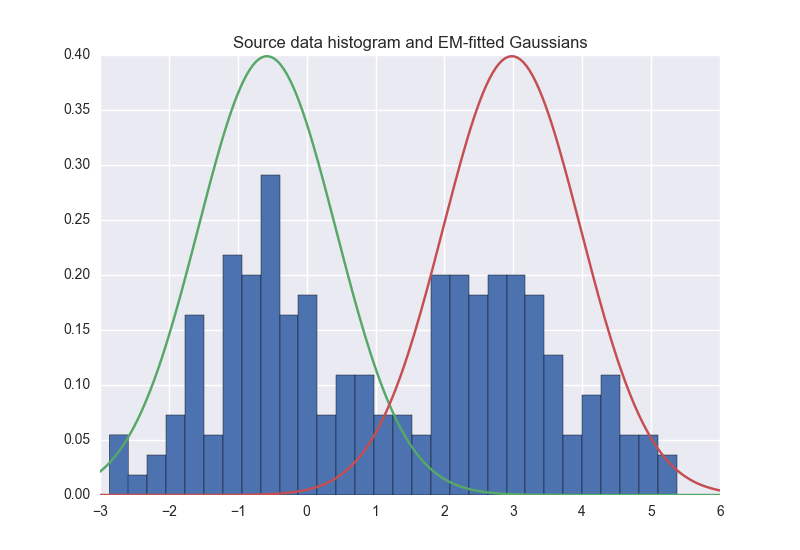
\includegraphics[width=0.8\linewidth]{img/visualization.png}
    \caption{Visualization of fitted gaussians and data histogram} \label{fig:visualization}
\end{figure}

\printbibliography
\end{document}
